\documentclass[10pt,twocolumn,letterpaper]{article}

    \usepackage{cvpr}
    \usepackage{times}
    \usepackage{epsfig}
    \usepackage{graphicx}
    \usepackage{amsmath}
    \usepackage{amssymb}
    
    % Include other packages here, before hyperref.
    
    % If you comment hyperref and then uncomment it, you should delete
    % egpaper.aux before re-running latex.  (Or just hit 'q' on the first latex
    % run, let it finish, and you should be clear).
    \usepackage[pagebackref=true,breaklinks=true,letterpaper=true,colorlinks,bookmarks=false]{hyperref}
    
    \cvprfinalcopy % *** Uncomment this line for the final submission
    
    \def\cvprPaperID{****} % *** Enter the CVPR Paper ID here
    \def\httilde{\mbox{\tt\raisebox{-.5ex}{\symbol{126}}}}
    
    % Pages are numbered in submission mode, and unnumbered in camera-ready
    \ifcvprfinal\pagestyle{empty}\fi
    \begin{document}
    
    %%%%%%%%% TITLE
    \title{Context-based Pedestrian Path Prediction}
    
    \author{Yasheng Sun\\
    117020910076\\
    {\tt\small sunyasheng123@gmail.com}
    % For a paper whose authors are all at the same institution,
    % omit the following lines up until the closing ``}''.
    % Additional authors and addresses can be added with ``\and'',
    % just like the second author.
    % To save space, use either the email address or home page, not both
    }
    
    \maketitle
    %\thispagestyle{empty}
    
    %%%%%%%%% ABSTRACT
    \begin{abstract}
    This project focus on intention prediction of pedestrians when they cross
    the road through Dynamical Bayesian Network. The insight is that 
    the futrue path of a pedestrian is usually relevant to the environment
    layout around him. Hence his model incorporates 
    situation awareness of pedestrian and the environment layout as latent 
    states to infer the changes of pedestrian dynamic state, which determines the
    trajectories of this pedestrian. This work involves
    a particular scenario where a crossing pedestrian might cross or stop at the
    curb. Experiment shows that we can anticipate the dynamic changes of this pedestrian
    ahead of event and therefore predicts a more accurate path with this model. All 
    code are publicly available on my github \url{https://github.com/sunyasheng/Bayesian-Statistics-Assignment}.

    \end{abstract}
    
    %%%%%%%%% BODY TEXT
    \section{Introduction}
    Self-driving has made a significant progress in these years while many automated
    car has traveled on the road for a tested driving. The safety of pedestrians 
    plays an important role in the decision making process of self-driving car. 
    Accurate pedestrian path prediction is a prerequisite for the car to navigate
    through the crowd without threatening the safety of pedestrians. Accurate trajectory
    prediction is a challenging problem, since the dynamics of a pedestiran highly variable.

    An insight in this work is that the 
    environment layout surrounding him will affect his intention, which might be 
    reflected in his following action. We assume that the pedestrian decision
    is to large extent affected by three key parts: the existence of an approaching
    vehicle on collision course, the pedestrian's awareness and the spatial
    layout of environment. Therefore, the Dynamic Bayesian Network(DBN) is proposed to 
    integrate these parts into an unified framework. The DBN captures these three 
    factors as latent states working on top of a Switching Linear Dynamic System(SLDS),
    hence controlling the dynamics of the pedestiran. 

    Bayesian Network models the causal relationship by a directed graph, which
    can be utilized to describe the cause and affect of pedestrian action or 
    the environment context in a probabilistic fashion. For instance, the pedestrian
    is less likely to cross the road if the car drives with a high speed in this
    critical situation. Or the pedestrian tends to cross if he does not even notice
    the driving car. Those relationships can be modeled by a conditional probability
    which is presented as an edge in the Bayesian Network. Situation criticality
    is estimated by the expected minimum distance of the pedestrian and the vechicle
    at the closest approach in future. Situation awareness represents whether or not
    this pedestrian has seen the vehicle up to now, which is estimated through 
    his head orientation of past time. Spatial layout is described by
    the distance to the curbside. The observables(see the shaded node in Fig.~\ref{dbn})
    i.e. expected distance at closest approach, pedestrian position, head orientation,
    curb location, are measured by the external sensors.
    
    Since the state of pedestrian 
    changes evolving with time slices, the Dynamic Bayesian Network(DBN) is utilized here
    to reflect the state evolution with timestamps. All the parameters in DBN are learned
    by the annotated data in a supervised learning fashion.




    \begin{figure}[t]
        \begin{center}
           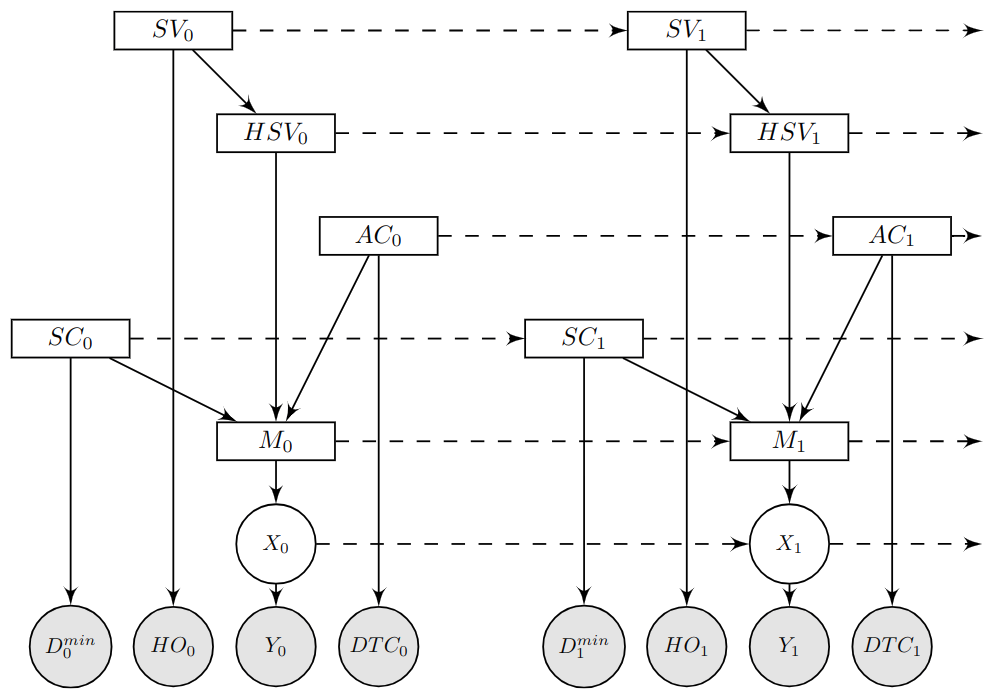
\includegraphics[width=1.0\linewidth]{images/dbn.png}
        \end{center}
           \caption{The DBN framework unrolled in two time slices, rectangle/circle/shaded
           nodes are discret/continous/observed variables.}
        \label{fig:long}
        \label{fig:onecol}
        \label{dbn}
    \end{figure}
    

    \section{Methodology}
    Our goal is to devise a model that can successfully anticipate the dynamic of the 
    pedestrian through the context information. The dynamic is the switching state in
    SLDS, which indicates the basical motion model used at each time instance.
    We argue that the decision of pedestrian to stop at the curb or cross the street is 
    highly influenced by his awareness of situation, his position with respect to
    the curbside and the existence of an approaching vehicle on collision course. Hence, the 
    DBN is proposed to capture these three factors as latent state which affects the 
    switching state in Switching Linear Dynamic System(SLDS) as shown in Figure~\ref{dbn}. 

    \subsection{Graphical Model}
    The proposed DBN is shown in Fig.~\ref{dbn}. Those variables can be split into 
    two sets: one set related to SLDS that consists of switching state $M$, latent position
    state $X$ and associated observation $Y$ while another one relating to the scene 
    context information including spatial layout, situation criticality
    and the pedestrian's awareness($Z = \{SV, HSV, SC, AC\}$), which influences the switching
    state $M$ in SLDS and associated observables $E=\{HO, D^{min}, DTC\}$. \\


    \noindent
    \textbf{SLDS}. The SLDS consists of a continous hidden state $X_t$, a discret
    switching state $M_t$ and the observation of the state $Y_t$ with observation 
    noise $N(0,R)$.  Two motion types are involved at any time instances in this secenario, including 
    walking($M_t=m_w$) and standing($M_t = m_s$). The velocity in standing motion type is
    zero while the velocity in walking motion type is $v_t$. A person's lateral position
    at time $t$ is denoted by $x_t$. Formally, the motion dynamics is illustrated as
    \begin{eqnarray*}
        x_t = x_{t-1} + v_t + \epsilon\\
        v_t = \left\{
            \begin{array}{lr}          0 & M_t = m_s \\
                                    v^{m_w} & m_t = m_w
            \end{array}
        \right.
    \end{eqnarray*}

    Here we assume zero-mean process noise $\epsilon \sim N(0, Q)$ and also the fixed 
    time interval $\Delta t= 1$. The velocity can also be included in this dynamic 
    system such that the state can be described as $X_t = [x_t, v_t^{m_w}]^T$.
    \begin{eqnarray*}
        X_t = A^{(M_t)}X_{t-1} +  \left[\begin{matrix}
            \epsilon  \\
            0 
           \end{matrix}\right] & \epsilon_t \sim N(0, Q)\\
        Y_t = CX_t + \mu_t & \mu_t \sim N(0, R)
    \end{eqnarray*}
    where the switching state determines the linear state transformation matrix $A^{(m)}$,
    \begin{eqnarray*}
        A^{m_s} = \left[ \begin{matrix}
            1&0\\
            0&1
        \end{matrix}
            \right]  
        A^{m_w} = \left[ \begin{matrix}
            1&1\\
            0&1
        \end{matrix}
            \right]  
    \end{eqnarray*}
    The lateral position $Y_t \in R$ is the observation with the observation matrix
    $C$ = [1 0]. Therefore, the conditional probability distributions of this graphical 
    model can be described as $P(X_t|X_{t-1}, M_t) = N(X_t|A^{(M_t)}X_{t-1},Q)$ and
    $P(Y_t|X_t) = N(Y_t|CX_t,R)$.\\


    \noindent
    \textbf{Context}. The transition probability of the switching state $M_t$ in SLDS is 
    conditioned on the current context information $SC_t, HSV_t, AC_t$ and 
    previous switching state $M_{t-1}$. Formally, 
    \begin{eqnarray*}
        P(M_t|M_{t-1}, SC_t, HSV_t, AC_t)
    \end{eqnarray*}
    Essentially, this is a switching state transition table parameterized by $SC_t, HSV_t, AC_t$.
    This temporal transition of context state $SC, HSV, AC$ can be factorized to
    \begin{eqnarray*}
        P(SC_t, HSV_t, AC_t|SC_{t-1}, HSV_{t-1}, AC_{t-1}) = \\
        P(HSV_t|HSV_{t-1},SV_t)\times P(SV_t|SV_{t-1}) \\
         \times P(SC_t|SC_{t-1}) \times P(AC_t|AC_{t-1})
    \end{eqnarray*}
    where the lalent variable $SV$ indicates whether the pedestiran sees the vehicles at
    current time step. $HSV$ indicates whether the pedestrian is aware that the vehicle approaches.
    $HSV$ should be true if the pedestrian sees the vechicle for some $t'\leq t$. 
    \begin{equation*}
        P(HSV_t|HSV_{t-1}, SV_t) = 
        \left\{
            \begin{array}{lr}  
                1 & HSV_t = (HSV_{t-1} V SV_t)\\  
                0 & otherwise
                \end{array}
        \right.
    \end{equation*}
    The transition probability of $HSV_t$ can be defined simply the logical $OR$ between 
    the Boolean $HSV_{t-1}$ and $SV_t$ variables.

    The latent variable $SC$ indicates the criticality of the situation if both the pedestrian 
    and the vehicle continue approaching with their current velocities. $AC$ indicates whether
    the pedestrian is currently on a position near the curbside since the curbside is usually 
    where he chooses to wait or delay his crossing behavior. Similarly, the $SV$, $SC$ and $AC$
    varaibles also depend on their previous value at last time instance, which is designed for 
    the smoothness of those latent variables.  

    The observations obtained by sensors serve as evidence for the latent context variables 
    $SV, SC, AC$. The observation probability distribution can also be factorized to
    \begin{eqnarray*}
        P(HO_t|SV_t)\times P(D_t^{min}|SC_t) \times P(DTC|AC_t)
    \end{eqnarray*}

    The head orientation observation variable $HO_t$ provides evidence for the latent $SV$
    variable. $HO_t$ is a vector which captures the classifier responses in certain 
    looking direction. Multiple classifiers has been trained to identify the looking direction
    of the pedestrian through the image of his head. The values conform to different
    distributions across classes conditioned on whether the pedestiran sees the vechicle $SV$.
    The $HO_t$ here is hence modeled as a Multinomial distribution conditioned $SV_t$ with $p_{sv}$
    as parameter vector.
    \begin{eqnarray*}
        P(HO_t|SV_t = sv) = Mult(HO_t|p_{sv})
    \end{eqnarray*}

    The expected minimum distance between the pedestiran and vehicle is taken as the evidence
    to estimate the situation criticality $SC$, if they continue approaching with their current
    velocities. It seems that the assumption is navie, but it provides the information to
    measure how critical this situation is. The gamma distribution is used here to describe
    $D^{min}$ conditioned on $SC$ with the shape parameter $a$ and scale parameter $b$. 
    \begin{eqnarray*}
        P(D_t^{min}|SC_t=sc) = \Gamma(D_t^{min}|a_{sc}, b_{sc})
    \end{eqnarray*}

    The At-Curb variable $AC$ is measured by the distance between the lateral position of the
    pedestrian and the position of the curb ridge. The position of curb is obtained by the image processing 
    procedure. And the position of the pedestiran is the filtered expected position $E[x_t]$ from the 
    Kalman Filter. Therefore, the Distance-to-Curb, $DTC$, is computed as the difference 
    between the filtered position of Kalman and and the curb position. Also it is worthy to 
    mention that the $DTC$ can be estimated even at future time instances using the predicted 
    position. The distribution of $DTC$ conditioned on $AC$ is modeled as a Normal distribution,
    \begin{eqnarray*}
        P(DTC_t | AC_t = ac) = N(DTC_t|\mu_{ac}, \sigma_{ac})
    \end{eqnarray*}
     

    \subsection{Inference}
    The DBN model works in a forward fashion to predict and filter the state when
    it receives the measurement from sensors at each time step. Exact inference in 
    this model is intractable since the exact posterior distribution will have $|M|^T$
    modes after $T$ time steps. Therefore here we use the Expectation Propogation~\cite{IEEEhowto:minka} technique
    to do approximate inference, where the posterior distribution is approximated by a 
    simple distribution through minimizing the KL divergence of the approximated and
    exact posterior distribution. Hence DBN consists of three main procedure for each 
    time instance: predict, update and collapse. 

    A prediction for time $t$ is denoted by $\bar{P}_t(\cdot)=P(\cdot|O_{1:t-1})$ before
    receiving the observation $O_t$, and updated estimate after observation receiving is 
    denoted by $\hat{P}_t(\cdot) = P(\cdot|O_{1:t})$. $\tilde{P}(\cdot)$  
    represents the approximated updated estimate which collapsed at each time instance $t$
    and will be passed to the predict module as input at time step $t+1$.\newline

    \noindent
    \textbf{Predict}
    The predicted posterior distribution$\tilde{P}_{t-1}(\cdot)$ after collapse serves as input of
    this time instance, including the joint distribution over latent motion and context nodes
    $\tilde{P}_{t-1}(X_{t-1},Z_{t-1})$ and the conditional Normal distribution
     $\tilde{P}_{t-1}(X_{t-1}|M_{t-1}) = N(X_{t-1}|\tilde{\mu}_{t-1}^{(M_{t-1})}, \tilde{\Sigma_{t-1}^{M_{t-1}}})$.
    Here we use $Z_t$ to represent ${HSV_t, SV_t, SC_t, AC_t}$.
    The joint probability of latent variables in previous and current time steps is computed based on
    the transition probability we trained. 
    \begin{eqnarray*}
        \bar{P}_t(M_t, M_{t-1}, Z_t, Z_{t-1}) =\\
         P(M_t|M_{t-1}, Z_t)P(Z_t|Z_{t-1})\tilde{P}_{t-1}(M_{t-1}, Z_{t-1})
    \end{eqnarray*}
    For continous state $X_t$ we condition on all the possible models $M_t$ to predict the effect
    of models $M_t$. Formally, 
    \begin{eqnarray*}
        \bar{P}_t(X_t|M_t, M_{t-1}) =\\
         \int P(X_t|X_{t-1}, M_t) \times \tilde{P}_{t-1}(X_{t-1}|M_{t-1})dX_{t-1}
    \end{eqnarray*}

    \noindent
    \textbf{Update}
    The observation is incorporated in the update step to obtain the joint posterior. The likelihood
    term of observation follows the Kalman Filtering setting.
    \begin{eqnarray*}
        P(Y_t|M_t, M_{t-1}) = \int P(Y_t|X_t)\times \bar{P}(X_t|M_t,M_{t-1}) dX_t \\
        = N(Y_t|C\bar{\mu}^{(M_t,M_{t-1})}, \bar{\Sigma}_t^{(M_t, M_{t-1})} + R)
    \end{eqnarray*}
    And the updated $X_t$ also follows the standard Kalman Filtering setting conditioned on $|M|^2$ transition
    conditions. 
    \begin{eqnarray*}
        \hat{P}_t(X_t|M_t,M_{t-1}) \propto P(Y_t|X_t)\times \bar{P}_t(X_t|M_t,M_{t-1})
    \end{eqnarray*}

    The joint posterior of latent discret nodes are given by 
    \begin{eqnarray*}
        \hat{P}_t(M_t, M_{t-1}, Z_t, Z_{t-1})\propto P(Y_t|M_t, M_{t-1})\\
        P(E_t|Z_t)\bar{P}_t(M_t,M_{t-1},Z_t,Z_{t-1})
    \end{eqnarray*}
    Here the observation $E_t$ represents the $\{DTC_t, HO_t, D_t^{min}\}$

    \noindent
    \textbf{Collapse}
    To make this model tractable, the state of previous state need to be maraginalized out and only
    the varaibles at current time step are kept, which will be carried over to the next prediction step.
    \begin{eqnarray*}
        \tilde{P}_t(M_t,Z_t) = \sum_{M_{t-1}}\sum_{Z_{t-1}}\hat{P}_t(M_t, M_{t-1}, Z_t, Z_{t-1})
    \end{eqnarray*}
    The continous variable $X_t$ is also approximated by marginalizing the variable from previous time
    step. 
    \begin{eqnarray*}
        \tilde{P}_t(X_t|M_t) = \sum_{M_{t-1}} \hat{P}_t(X_t|M_t, M_{t-1})\times P(M_{t-1}|M_t) \\
        = N(X_t|\tilde{\mu}_t^{(M_t)}, \tilde{\Sigma}_t^{(M_t)})
    \end{eqnarray*}
    The parameters $(\tilde{\mu}_t^{(M_t)}, \tilde{\Sigma}_t^{(M_t)})$ are calculated through minimizing
    the KL divergence between exact positerior and approximate posterior~\cite{IEEEhowto:minka} under
    the constraint that the approximate posterior distribution is Normal Distribution.
    The $P(M_{t-1}|M_t)$ is obtained by marginalizing and normalizing $\hat{P}_t(M_t, M_{t-1}, Z_t, Z_{t-1})$

    \section{Experiment}

    \subsection{Dataset Description}
    \begin{table}
        \begin{center}
            \begin{tabular}{|l|c|}
                \hline
                Context & Sequence Number\\
                \hline
                \hline
                Not SC, SV, Crossing & 14\\
                Not SC, not SV, Crossing & 9\\
                SC, not SV, Crossing & 11\\
                SC,SV,Stopping & 14\\
                SC,SV,Crossing & 10\\
                \hline
            \end{tabular}
        \end{center}
        \caption{The detail of dataset statistics.}
        \label{Statistics}
    \end{table}
    The dataset comes from a publicly available dataset~\cite{IEEEhowto:kooij,IEEEhowto:data} which 
    is annotated by Daimler Company for self-driving research.

    This dataset~\cite{IEEEhowto:data} includes 58 sequences recorded by a stereo camera involving single pedestrian
    with intention to cross the road, which features different situation criticalities(critical,
    vs. non-critical), pedestrian behavior(crossing vs. stopping at the curb) and pedestrian
    situational awareness(seen vehicle vs. not seen vehicle). The detail of this dataset statistics is 
    shown in Table.~\ref{Statistics}. There are five sub-scenarios in this dataset, four of which
    represent normal pedestrian behaviros while the last sub-secenario is anomalous since 
    the pedestrian choose to cross even though he is aware of the critical situation. For framework synchronization sequences
    are labeled with time-to-event(TTE) values. TTE is defined to be 0 when the pedestrians step
    on the ground at the curbside. Frames before/after TTE = 0 have negative/positive values.

    Position ground truth(GT) comes from manual labeling of the pedestrian bounding boxes and the 
    median disparity of the upper pedestiran body area is calculated. A mean gait cycle consumes 
    17.3 frames(1.0s) with 1.6 frames(0.1s) standard deviation from the analysis of the trajectories.


    The positional observation $Y_t$ is estimated by the resulting bounding boxes extracted from 
    HOG/linSVM detector and has compensated the vehicle ego-motion. The detector takes as input
    region of interests provided by the obstacle detection module using dense stereo data. Then
    the bounding box is extracted by the detector and the median disparity is calculated to 
    estimate the position of the pedestiran.

    The angle of observed head orientation $HO_t$ is discretized to eight orientation classes
    of $0^\circ, 45^\circ,\cdots, 315^\circ$. The detector for each class is trained, i.e. 
    $f_0,\cdots, f_{315}$, so the response of the detector $f_o(I_t)$ serves the evidence
    that the region of interest contains the head orientation of orientation class $o$.
    In more detail, every detector is a neural network trained in a $one-vs-rest$ fashion.
    For detection, regions of interest are proposed 
    from disparity based image segmentation and the most likely head image region $I^\star$
    is selected to rescale to $16 \times 16px$ before classification. The output of classifier
    is the response strength $HO_t = [f_0(I_t^{\star}), \cdots, f_{315}(I_t^{\star})]$ over 
    different discretized head orientation.

    Fig.~\ref{head_measure} shows a sequence where the pedestrian crosses the road 
    when the situation is not critical. From the figure we can see that the pedestrian
    sees the approaching vechicle($SV=True$) when his head angle is in the range of
    $\pm 45^{\circ}$ at about $t=10$ hence the $HSV = True$ since that time.   

    \begin{figure}[t]
        \begin{center}
           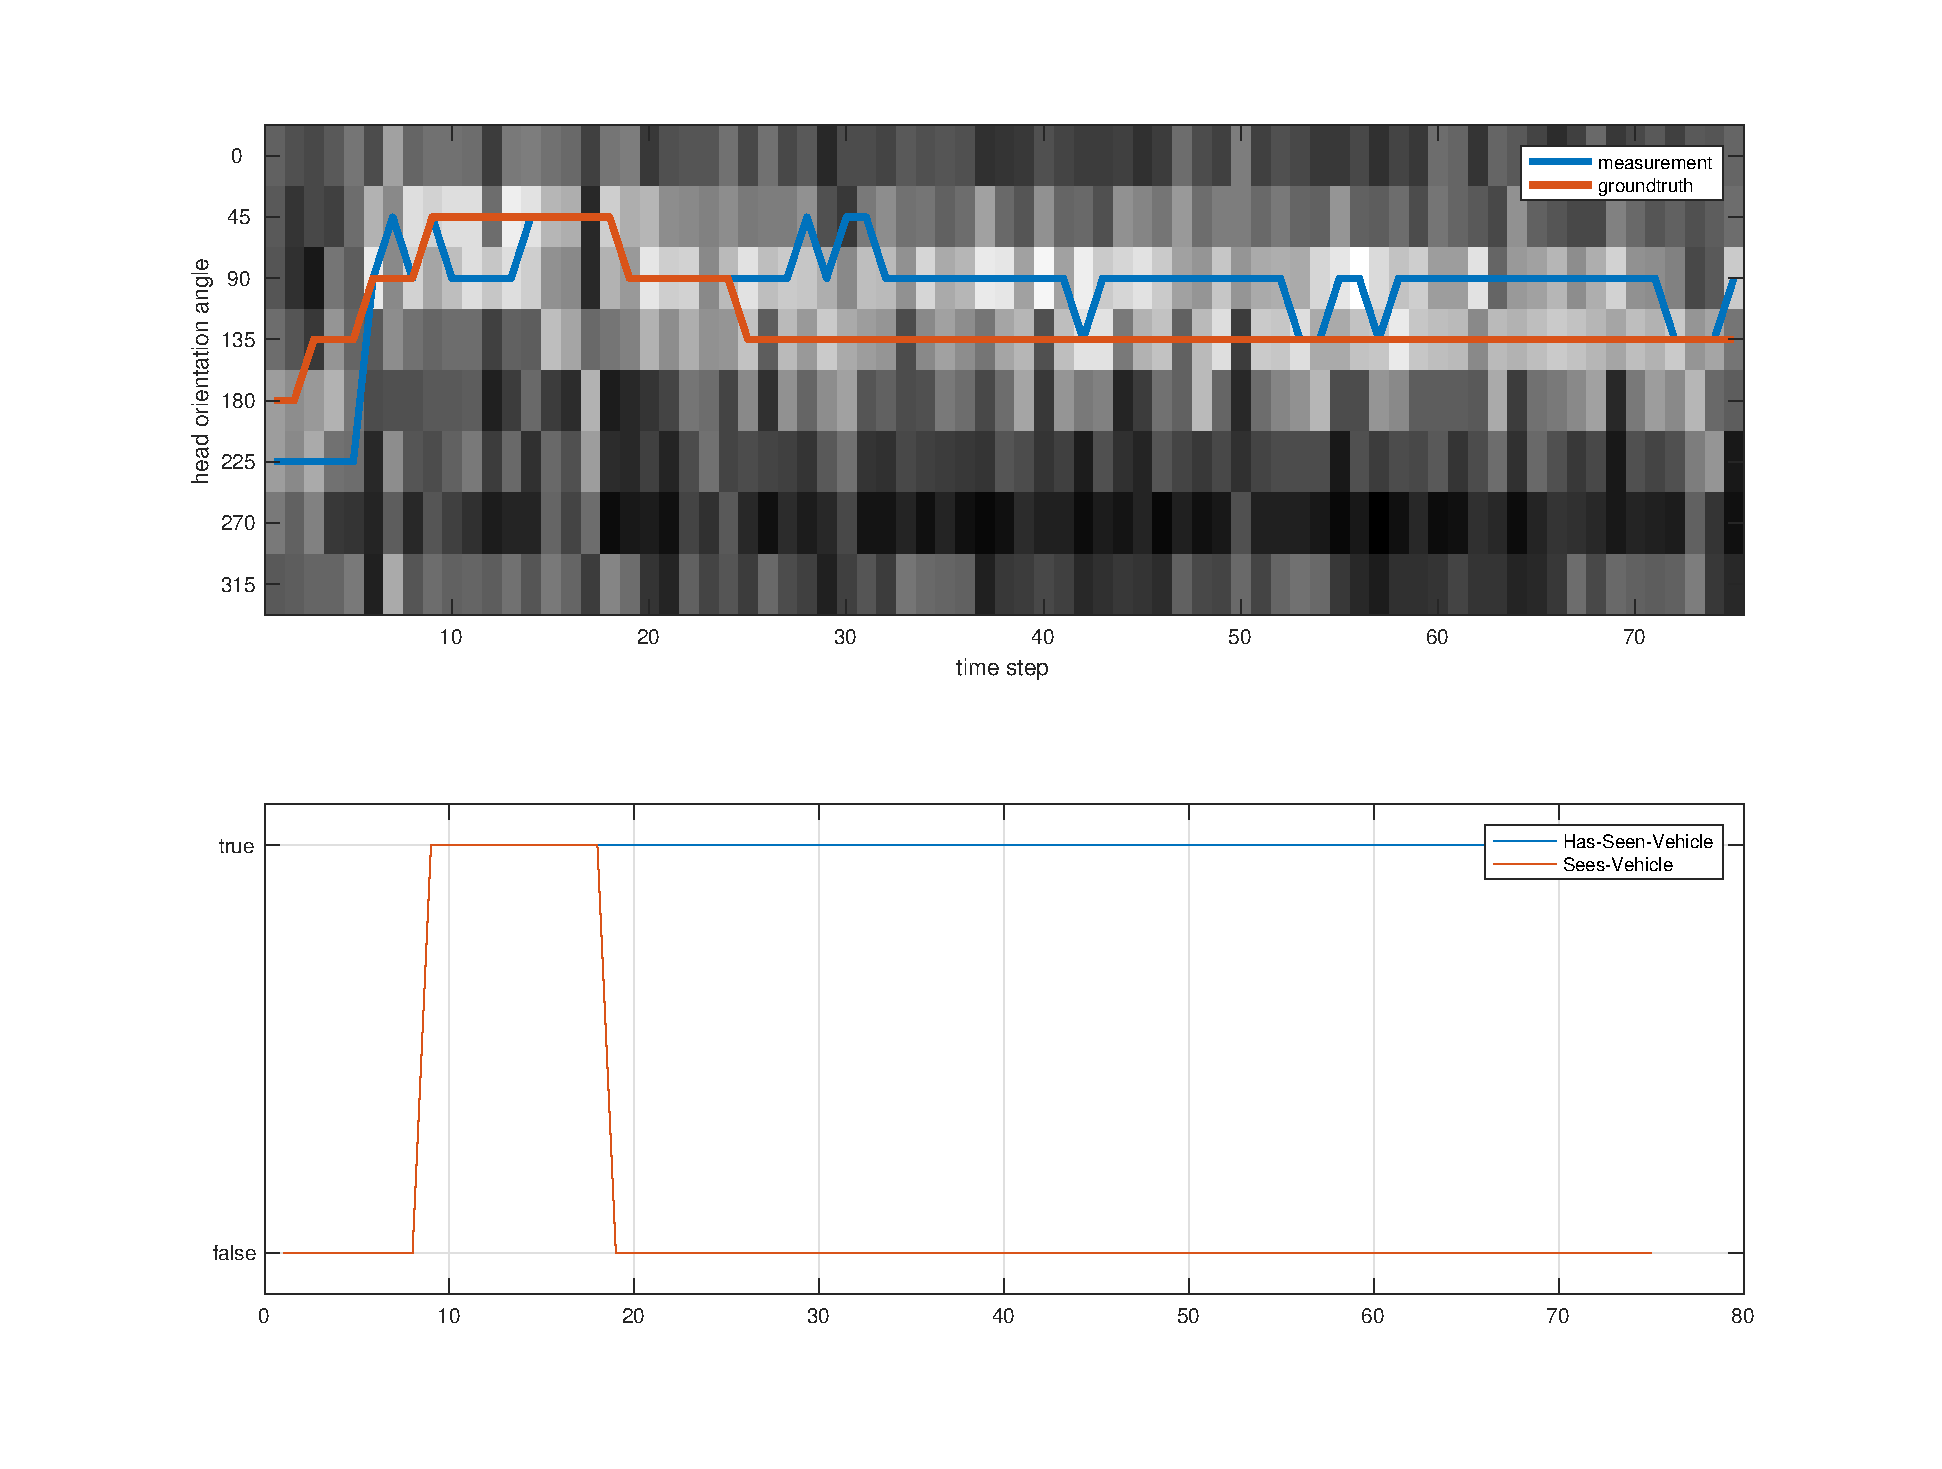
\includegraphics[width=1.1\linewidth]{images/ho.eps}
        \end{center}
           \caption{The head measurement and groundtruth of a crossing pedestrian.}
        \label{fig:long}
        \label{fig:onecol}
        \label{head_measure}
    \end{figure} 
  

    The expected minimum distance $D^{min}$ between vehicle and pedestrian is calculated 
    at each time step based on the current position and velocity. Vehicle speed is obtained
    through on-borad sensors and pedestrian velocity is approximated by the first order
    of derivative over the last 10 frames. For distance to curb($DTC$), the curbside is detected
    by Hough transform. $Y_t^{curb}$ is then estimated by the mean lateral position of detected 
    line. 
    

    The ground truth GT switching state $M_t = m_s$ when TTE $>=$ 0, and $M_t = m_w$ at all
    other moments for the stopping sequences. For the crossing sequences, $M_t = m_w$ 
    at all time steps. 

    For head obaservation $HO$, we assume that the pedestrian is aware of($SV = True$) an approaching vehicle
    if the GT head orientation is in a range of $\pm 45^{\circ}$ centered angle $0^{\circ}$(the 
    direction of head pointing towards the camera) and does not see($SV = False$) the vechicle for angles outside
    this range. 
    The distribution $\Gamma(D^{min}|a_{sc}, b_{sc})$ of observation $D^{min}$ is estimated 
    over situation critical $SC$ labels, which is set once for all time instances
    per sequence. The distribution $N(DTC_t|\mu_{ac},\sigma_{ac})$
    is estimated from GT curb positions and GT pedestrian positions over at curb $AC$ labels, 
    which are set to $AC_t$ = true if $-1\leq TTE \leq 1$ in crossing sequences or $TTE \geq -1$
    in stopping sequences.

    
    \subsection{Training Details}
    In this section, we introduce training details of the conditional probability distribution  
    computation.
    Two kinds of probability distribution is required to be estimated, including the 
    transition probability between adjacent time slices and the emission probability
    at the same time instance. 
    
    \noindent
    \textbf{Transition Probability} 
    \begin{eqnarray*}
        P(SV_t|SV_{t-1}) = \frac{\sharp(SV_t, SV_{t-1})}{\sharp(SV_{t-1})}
    \end{eqnarray*}
    \begin{eqnarray*}
        P(SC_t|SC_{t-1}) = \frac{\sharp(SC_t, SC_{t-1})}{\sharp(SC_{t-1})}
    \end{eqnarray*}
    \begin{eqnarray*}
        P(AC_t|SC_{t-1}) = \frac{\sharp(AC_t, AC_{t-1})}{\sharp(AC_{t-1})}
    \end{eqnarray*}
    \begin{eqnarray*}
        P(M_t|M_{t-1}, SC_t, HSV_t, AC_t) = \\
         \frac{\sharp(M_t,M_{t-1}, SC_t, HSV_t, AC_t)}{\sharp(M_{t-1}, SC_t, HSV_t, AC_t)}
    \end{eqnarray*}

    Those conditional probability distribution is approximated by the fraction of
    existence frequency of the joint variables over marginal variables. Note that 
    the $SC$ labels are only set once in real dataset, so we fix the SC situation 
    probability to 1/100 for the changing state.
    

    \noindent
    \textbf{Emission Probability}
    \begin{figure}[t]
        \begin{center}
           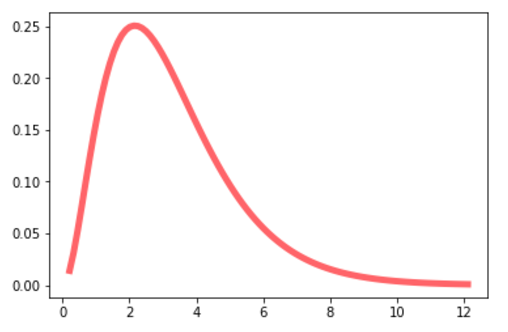
\includegraphics[width=0.9\linewidth]{images/sc0.png}
        \end{center}
        \begin{center}
            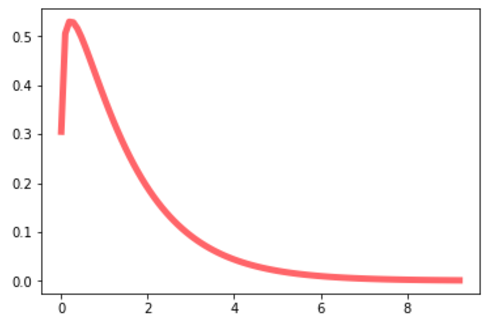
\includegraphics[width=0.9\linewidth]{images/sc1.png}
         \end{center}
        \caption{Probability distribution of minimum distance between pedestrian and vehicle. Upper
        figure is $\Gamma(D_t^{min}|a_{0}, b_{0})$ and Lower $\Gamma(D_t^{min}|a_{1}, b_{1})$.}
        \label{fig:long}
        \label{fig:onecol}
        \label{gamma}
    \end{figure}
    \begin{eqnarray*}
        P(HO_t|SV_t) = Multi(HO_t|p_{sv})
    \end{eqnarray*}
    The Head-Orientation $HO_t$ serves as evidence for Sees-Vehicle($SV_t$). $HO_t$ 
    is a vector which is the response over different classes of orientation. Hence 
    $HO_t$ is modeled as a sample from a Multinomial distribution conditioned on $SV_t$,
    with parameter vector $p_{sv}$. 
    The parameter vector $p_{sv}$ is estimated by the average of responses over different
    classes. 
    \begin{eqnarray*}
        P(D_t^{min}|SC_t = sc) = \Gamma(D_t^{min}|a_{sc}, b_{sc})    
    \end{eqnarray*}
    Situation-Critical $SC$ is infered by the minimum distance $D^{min}$ between 
    the pedestrian and vehicle under the constant velocity assumption, which indicates
    how critical the situation is and therefore lead to more accurate path prediction.
    The parameter is estimated by maximum likelihood estimation following~\cite{IEEEhowto:gamma}.
    Here we show the minimum distance $D^{min}$ distribution over the Situation-Critical($SC$)
    variable after MLE in Figure.~\ref{gamma}. The figure implies that usually the expected
    minimum distance is small under the critical situation, which conforms to our intuition.
    \begin{figure}[t]
        \begin{center}
           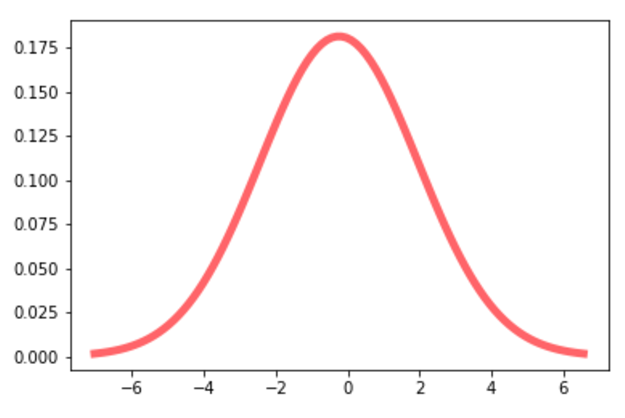
\includegraphics[width=0.9\linewidth]{images/ac0.png}
        \end{center}
        \begin{center}
            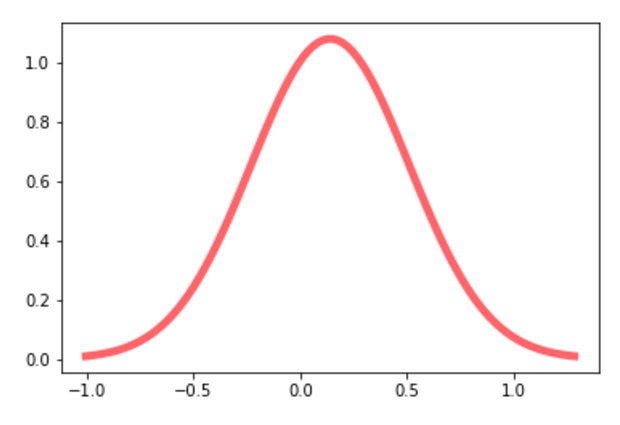
\includegraphics[width=0.9\linewidth]{images/ac1.png}
         \end{center}
        \caption{Probability distribution of distance between curb and pedestrian position. Upper
        figure is $N(DTC|\mu_{0}, \sigma_{0})$ and Lower $N(DTC|\mu_{1}, \sigma_{1})$.}
        \label{fig:long}
        \label{fig:onecol}
        \label{ac}
    \end{figure}
    \begin{eqnarray*}
        P(DTC_t|AC_t) = N(DTC_t|\mu_{ac}, \sigma_{ac})
    \end{eqnarray*}
    For At-Curb $(AC_t)$, we consider the Distance-To-Curb $DTC_t$. The expected
    lateral position of the pedestrian is obtained by the Kalman Filter in switching
    Linear Dynamic System while the location measure of the curb ridge is also
    filtered but by the constant position Kalman filter with zero mean process
    noise. The distribution is modeled as a Normal distribution with the mean
    $\mu$ and variance $\sigma$ needing to be learned. After MLE, the distribution
    is shown in Figure~\ref{ac}. The mean of distance 
    shows no difference in at-curb or not-at-curb situation, both located near 0. 
    But the variance is smaller in at-curb situation compared with the not-at-curb situation.

    \subsection{Evaluation}
    \begin{figure}[t]
        \begin{center}
            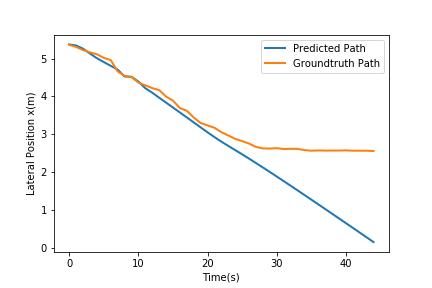
\includegraphics[width=0.95\linewidth]{images/lat_pos0.png}
        \end{center}
        \begin{center}
            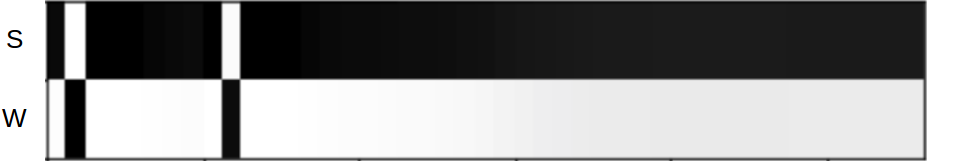
\includegraphics[width=0.85\linewidth]{images/m_bar_walk.png}
        \end{center}
        \begin{center}
            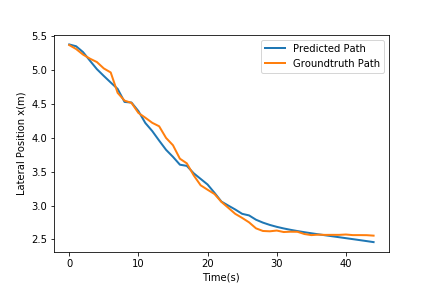
\includegraphics[width=0.95\linewidth]{images/lat_pos1.png}
         \end{center}
         \begin{center}
            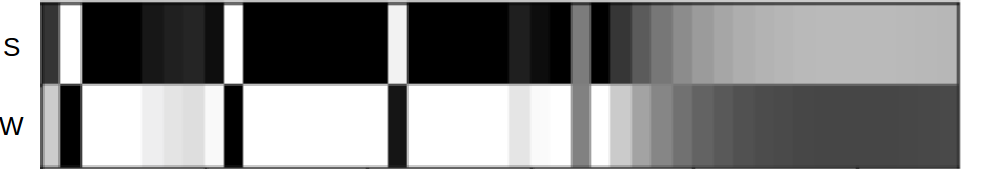
\includegraphics[width=0.8\linewidth]{images/m_bar_stop.png}
        \end{center}         
        \caption{The predicted lateral position and the groundtruth lateral position. 
        Upper figure shows the result predicted at TTE = -18(t=13) and lower figure shows 
        the result predicted at TTE = -4(t=27). The bar below represents the 
        probability of switching state in SLDS. The brighter the color of bar is, the higher
        probability it has.}
        \label{fig:long}
        \label{fig:onecol}
        \label{lat_pos0}
    \end{figure}
    Fig.~\ref{lat_pos0} illustrates a sequence from the stopping scenario in this fourth 
    row of Table.\ref{Statistics} where this pedestrian stops when he become aware
    of the critical situation. This pedestrian has not seen the vechicle and realize
    the critical situation at TTE = -18(t=13), hence the DBN model predicts that he will 
    continuing walking. It is reasonable that this model anticipate that the pedestrian 
    will continue walking at this time step 
    since there is no enough evidence showing the likelihood of stopping so far.
    But at TTE = -4(t=27), the strong evidence of having seen the vechicle,
    at curb and situation criticality is shown infered by the obaservation 
    hence the model predicts that the pedestrian is very likely to stop. So the predicted path is 
    very close to groundtruth benefitting from the correctly estimated motion $m_s$ state.
    The DBN enables more accurate and resonable path prediction using the information 
    from the context.

    \section{Summary}
    A novel model is proposed for pedestrian path prediction, which takes
    the context surrounding an ego-pedestrian into consideration. This DBN
    based model predicts the pedestrian path through SLDS with a latent 
    state controling the dynamics of pedestrian, which is determined by 
    the situation awareness, environmental spatial 
    layout and situation criticality. Experiment shows that the presented 
    model can predict the intention or dynamic of a pedestrian ahead of time, 
    thus we can predict the pedestrian path more accurately.

    This model can scale to more complicated scenario. Future work will involve 
    incorporation of of other secene context(e.g. interaction between pedestrians)
    and more flexible dynamics of pedestrians(e.g. acceration) instead of constant
    velocity assumption. 
    
    {\small
    \bibliographystyle{ieee}
    \bibliography{egbib}
    }
    \begin{thebibliography}{1}

    \bibitem{IEEEhowto:kooij}
    % H.~Kopka and P.~W. Daly, \emph{A Guide to \LaTeX}, 3rd~ed.\hskip 1em plus
    % 0.5em minus 0.4em\relax Harlow, England: Addison-Wesley, 1999.
    % D. Pathak, R. Girshick, P. Doll ́ ar, T. Darrell, and B. Hariha-ran.
    % Learning features by watching objects move. In \emph{CVPR}, 2017.
    Kooij, Julian Francisco Pieter, et al. Context-Based Pedestrian Path Prediction. Computer Vision – ECCV 2014. Springer International Publishing, 2014:618-633.
   
    \bibitem{IEEEhowto:data}
    \url{http://www.lookingatpeople.com/download-daimler-ped-predict-2014/index.html}
    
    \bibitem{IEEEhowto:gamma}
    \url{http://tminka.github.io/papers/minka-gamma.pdf}
    
    \bibitem{IEEEhowto:minka}
    Minka, and P. Thomas. "Expectation Propagation for approximate Bayesian inference." 7.7(2013):362-369.
    
    \bibitem{IEEEhowto:mh}
    \url{https://en.wikipedia.org/wiki/Metropolis-Hastings_algorithm}

    \bibitem{IEEEhowto:sunyasheng}
    \url{https://sunyasheng.github.io/}
    

    \end{thebibliography}

    \section{Appendix}

    In this section, we show another strategy MCMC(Markov Chain Mento Carlo) to calculate the posterior probability
    distribution of expected minimum distance($D_t^{min}$) between pedestrian and vechicle. 
    The new particle is obtained through random walk in traditional Metropolis-Hastings algorithm
    ~\cite{IEEEhowto:mh}. Since
    the dimension of varaibles is not independent and not isotropic, the random walk may 
    behave poorly~\cite{IEEEhowto:sunyasheng}. Here Adaptive Metropolis algorithm is introduced to 
    illustrate the covariance of the variables for a better proposed paritcle. Suppose that 
    the probability distribution of the proposed state is Normal distribution. 
    \begin{eqnarray*}
        p(x^\star \mid x_n) = N(x_n, \sigma^2 C_t)
    \end{eqnarray*} 
    The covariance can be illustrated as
    \begin{eqnarray*}
        Cov(X_0, X_1, ... , X_t) = \frac{\sum_{i=1}^{t-1}(x_ix_i^{T} - ((t-1)+1)\bar x_{t-1}\bar x_{t-1}^T)}{t}        
    \end{eqnarray*}
    where
    \begin{eqnarray*}
        \bar x_{t-1} = \frac{\sum_{i=0}^{t-1} x_i}{t}
    \end{eqnarray*}
    The $C_t$ can be updated at every time $t$ if we write the formula recursively.
    \begin{eqnarray*}
        C_{t+1} = \frac{(t-1)C_t}{t} + \frac{t\bar x_{t-1} \bar x_{t-1}^T - (t+1)\bar x_t \bar x_t ^T + x_t x_t^T}{t}
    \end{eqnarray*}
    Here the likelihood function is   
    \begin{eqnarray*}
        P(D_t^{min}|SC_t = sc) = \Gamma(D_t^{min}|a_{sc}, b_{sc})    
    \end{eqnarray*}
    It is conditioned on the Situation-Critical $SC$. There are two parameters in Gamma distribution $a_{sc}$ and $b_{sc}$.
    $a_{sc}$ is the location parameter and $b_{sc}$ is scale parameter. And we assume the prior probability of $a_{sc}$ 
    and $b_{sc}$ are positive numbers, which is subject to uniform distribution. Formally,
    \begin{eqnarray*}
        a_{sc} \sim U(0,\infty)\\
        b_{sc} \sim U(0,\infty)
    \end{eqnarray*}
    \begin{figure}[t]
        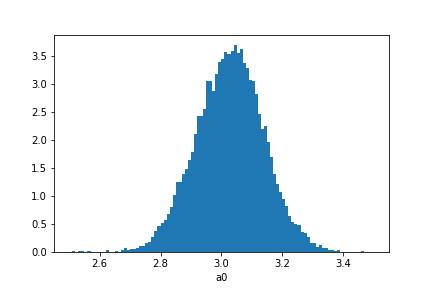
\includegraphics[width=0.49\linewidth]{images/a0.png}
        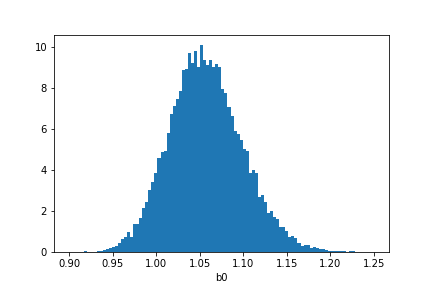
\includegraphics[width=0.49\linewidth]{images/b0.png}
        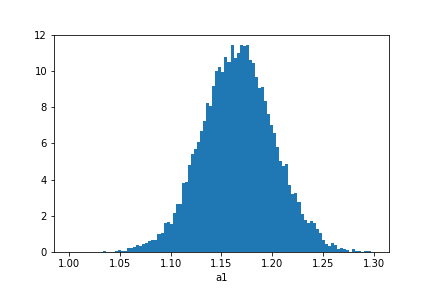
\includegraphics[width=0.49\linewidth]{images/a1.png}
        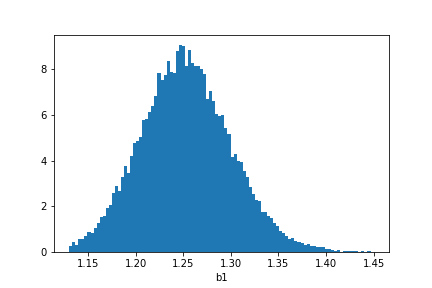
\includegraphics[width=0.49\linewidth]{images/b1.png}
        \caption{Posterior probability distribution of $a_{sc}$ and $b_{sc}$.}
        \label{fig:long}
        \label{fig:onecol}
        \label{post_gamma_sc}
    \end{figure}
    The posterior distribution of $a_{sc}$ and $b_{sc}$ after Adaptive Metropolis algorithm is shown in Figure.~\ref{post_gamma_sc}.

    Typically, the mean is $ab$ and the mode is $(a-1)b$ in Gamma density. The mode is 2.371 when $sc = 0$ and is 0.348 when $sc = 1$,
    which implies that expected distance $D_t^{min}$ between pedestrian and
    vechicle is closer when the situation is critical.
    And this posterior probability distribution is close to the distribution obtained by the Maximum Likelihood Estimation(MLE).
    For more implementation detail, please check my github \url{https://github.com/sunyasheng/Bayesian-Statistics-Assignment}. 
\end{document}